\chapter{IMPatienT : outil d’annotation et d’exploration de données multimodales de patients}

Dans un premier temps, nous avons développé \gls{impatient} (fig. \ref{fig:impatient_logo}) une application web qui permet l'annotation semi-automatique de compte rendu et d'images de biopsies musculaires. Cette application web, développée en 2020-2021, c'est à dire avant la mise à disposition des \gls{llms}, permet de créer un jeu de données structuré (tableau de patients) à partir de données non structurées (texte libre et images). Ainsi dans ce contexte-là, pour exploiter des données sous la forme de texte libre, il est nécessaire de procéder à son annotation manuelle afin de les structurer. L'objectif d'\gls{impatient} est de mettre à disposition une interface qui permet la numérisation de ces données non structurée, de les préparer pour l'application des méthodes de \gls{ml} traditionnelles et de fournir des outils d'explorations automatiques.


Pour structurer ces données biomédicales, nous utilisons une approche basée sur le concept d'ontologie: un vocabulaire standardisé pour décrire de manière unifiée les observations réalisées. S'il existe déjà des ontologies pour nommer les maladies (\gls{ordo}), les observations cliniques (\gls{hpo}), et des nomemclatures pour les gènes et mutations (HUGO, \gls{hgvs}), il n'existe aucune ontologie à ce jour permettant de décrire les observations histopathologiques dans les biopsies musculaires. Pour cela, \gls{impatient} intègre un module permettant en premier lieu la création de vocabulaire standard, que nous avons utilisé pour créer un vocabulaire standard des observations histopathologiques. Ensuite à partir de ce vocabulaire standard nous avons développé un module pour numériser et détecter de manière semi-automatique les termes du vocabulaire standard dans les comptes rendus de biopsies. Pour ajouter à l'aspect multimodal, nous avons développé un module de segmentation d'images assisté par intelligence artificielle. Ce module permet de rapidement annoter des images de biopsies avec les  termes du vocabulaire standard afin de créer un jeu données annoté qui permet l'entrainement d'IA de segmentation d'images automatique. Enfin, un dernier module de visualisation des données enregistrées permet d'explorer en temps réel les données de patient numérisées dans l'application web.

\begin{figure}[H]
  \centering
  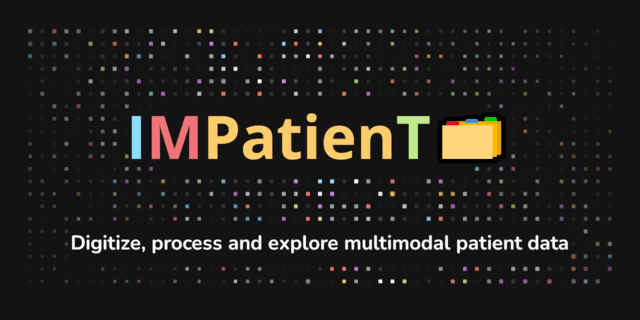
\includegraphics[width=0.7\textwidth]{figures/impatient_banner.png}
  \caption[Logo IMPatienT]{\textbf{Logo d’IMPatienT}}
  \label{fig:impatient_logo}
\end{figure}


\section{Manuscrit} 
Le manuscrit d'\gls{impatient} a été soumis à la revue scientifique  \textit{"Journal of Neuromuscular Diseases"} et  est présenté ci-dessous.

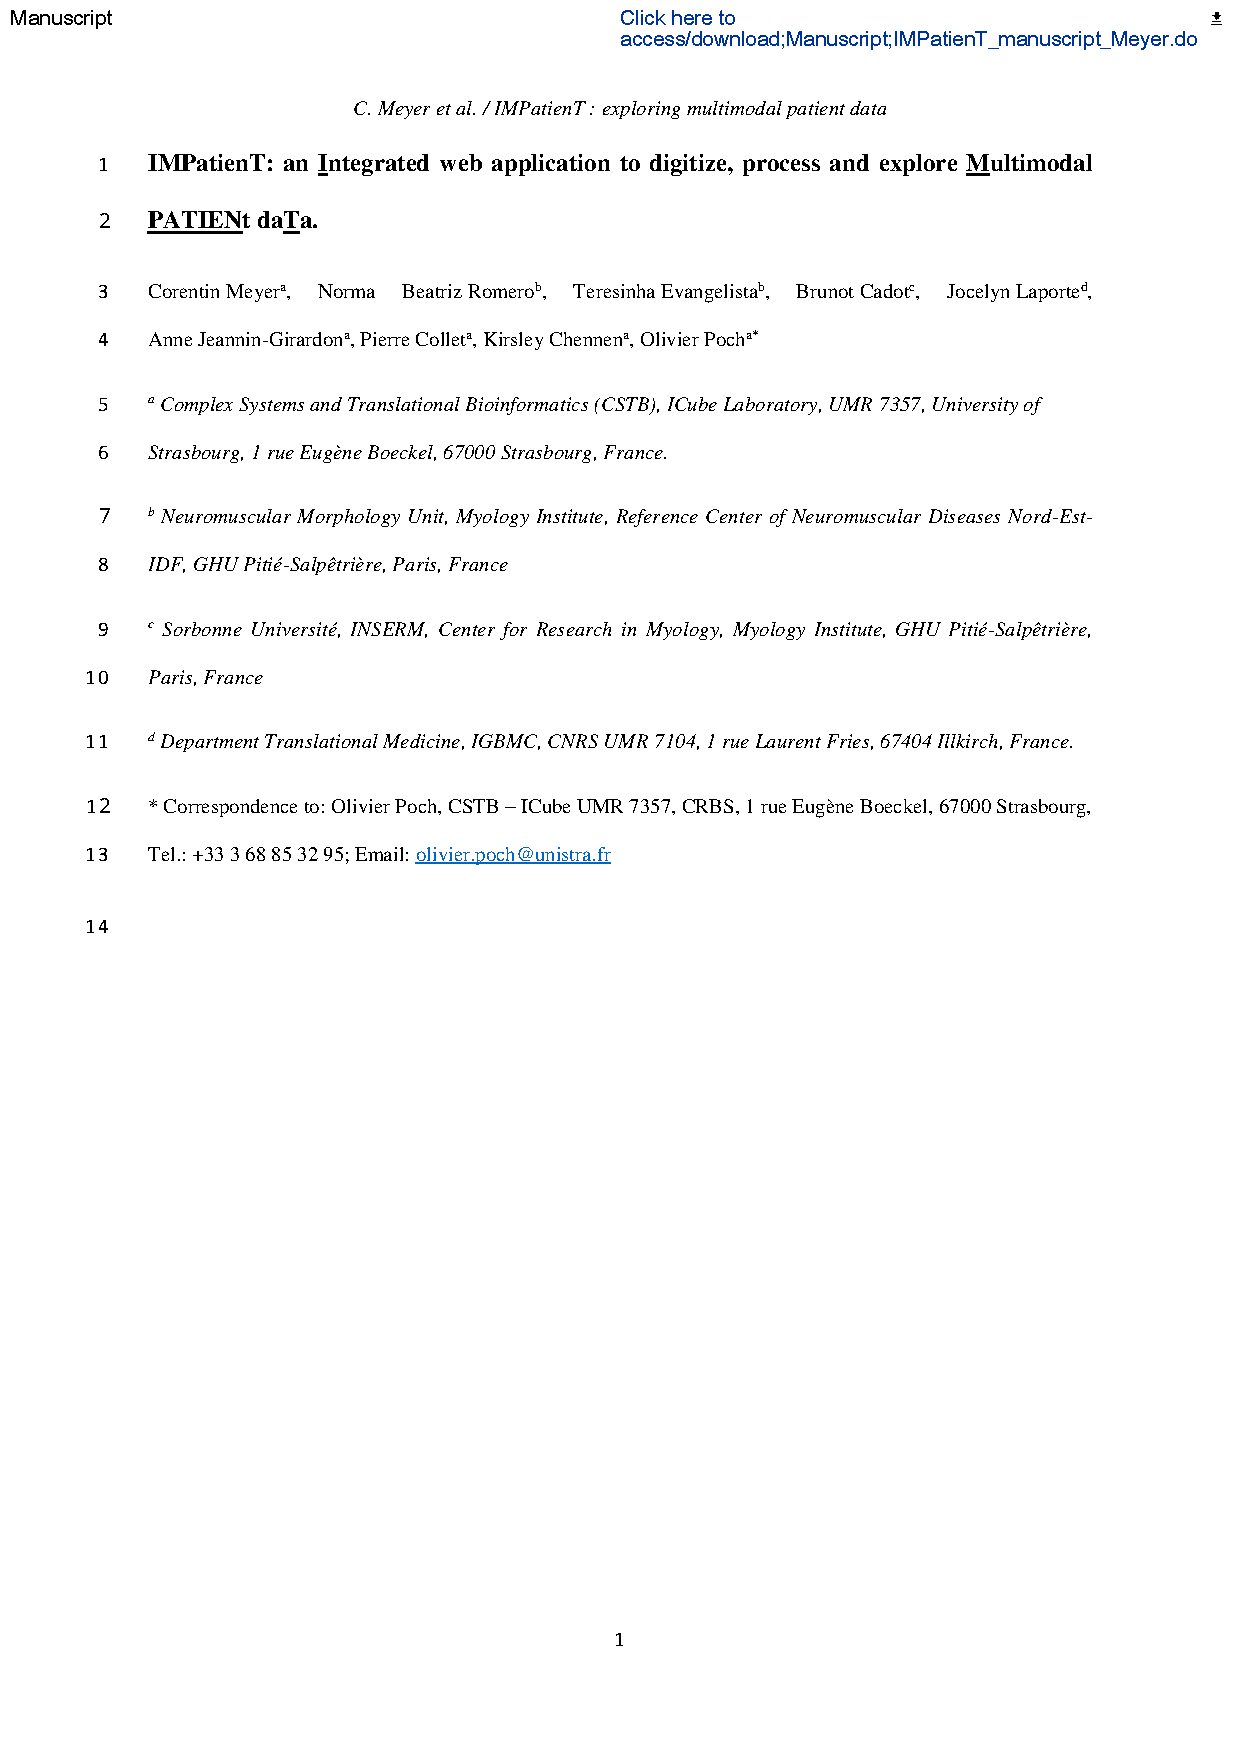
\includepdf[pages={1-27},scale=1,dpi=300]{corps/IMPatienT_pdf.pdf}


\section{Données sensibles et déploiement de la plateforme}
Afin de traiter les données de patients atteints de \gls{mc} (qui doivent rester privées), mais aussi de pouvoir faire une démonstration technique de l'outil, nous avons mis en ligne deux instances de la plateforme. Une première instance publique, à l'adresse \url{https://impatient.lbgi.fr}, contient une quarantaine de rapports de comptes rendus fictifs générés aléatoirement. Cette instance est accessible à tout le monde et est remise à zéro chaque jour. Une seconde instance privée, à l'adresse \url{https://myoxia.lbgi.fr}, contient 89 rapports de comptes rendus de patients provenant de l'Institut de Myologie de Paris qui ont été numérisés. Cette instance n'est accessible que par mot de passe et son contenu est sauvegardé de manière régulière. Le code source d'\gls{impatient} est \textit{open-source} et disponible dans un répertoire GitHub à l'adresse: \url{https://github.com/lambda-science/IMPatienT}.


\section{Limitations et perspectives de développement}
\gls{impatient} est une application web permettant d'annoter et d'explorer les données biomédicales issues de la biopsie musculaire de patients atteints de \gls{mc}. Cette application web a été développée pour pallier au manque d'outils permettant d'annoter et d'extraire de l'information de comptes rendus médicaux en texte libre grâce à une approche basée sur les ontologies. En plus d'intégrer les ontologies médicales déjà existantes (\gls{ordo}, \gls{hpo}, HUGO, \gls{hgvs}), \gls{impatient} permet de créer facilement un vocabulaire standard similaire à une ontologie pour les domaines où il n'existe pas encore d'ontologie de référence. Dans notre cas, nous l'avons utilisé pour créer notre propre vocabulaire standard des observations histopathologiques réalisées dans les biopsies musculaires. Nous avons passé en revue l'ensemble des 89 comptes rendus de biopsies musculaires et nous avons extrait et hiérarchisé par colorations les termes uniques trouvés dans ces rapports. Ce travail réprésente un total de 175 termes extraits composant notre vocabulaire standard.


Cependant, l'approche développée conçue pour l'annotation est semi-automatique et requiert donc toujours un travail manuel et humain de correction et de validation des annotations. Cette limitation empêche donc le passage à l'échelle et le traitement d'une masse importante de comptes rendus textuels ou d'images. De plus, l'approche utilisée est dépendante de la définition d'un vocabulaire standard exhaustif. Si un terme nouveau est présent dans un compte rendu et est absent du vocabulaire au moment de l'annotation, il faut le rajouter au préalable. De même, si on opère des modifications importantes du vocabulaire standard, il est peut-être nécessaire de devoir passer en revue l'ensemble des comptes rendus déjà numérisés pour vérifier si de nouveaux termes sont à associer aux comptes rendus ou si d'anciennes annotations sont à supprimer.


En termes de développement futur, il est nécessaire d'intégrer à \gls{impatient}  de nouveaux outils permettant l'automatisation de l'analyse des comptes rendus, par exemple un outil permettant de préremplir les formulaires avec les informations générales détectées. Ainsi, grâce aux récentes avancées dans le traitement de texte libre, notamment grâce aux\gls{llms}, nous avons développé de nouvelle méthode qui permettent d'automatiser ce processus d'annotation. Ces nouvelles méthodes sont décrites dans le chapitre 7: "NLMyo : Traitement de rapports textuels par LLMs". Il serait intéressant aussi de proposer des alternatives plus automatiques au système d'annotation avec le vocabulaire standard.


De plus au niveau de l'analyse d'images, il est intéressant de proposer un outil capable de quantifier grâce à l'\gls{ia} des marqueurs pathologiques dans les images de biopsie, car cette information est manquante dans les comptes rendus de biopsie, les observations ne sont que qualitatives et non quantitatives. Pour cela, nous avons développé un outil présenté dans le chapitre 8 "Vers une génération de rapports automatiques à partir d’imagerie avec MyoQuant".


Grâce à l'intégration de ces outils, l'application web\gls{impatient} deviendrait le socle de l'intégration de plusieurs outils d'\gls{ia} pour l'analyse de données multimodales. \gls{impatient} serait alors le point d'entrée mettant à disposition des outils pour créer une base de données multimodales de patients et fournir les outils adaptés à leur analyse et exploration.